In this module you will learn
\begin{itemize}
	\item how to sketch a phase portrait for a linear system of ODEs with constant coefficients
	\item how to use a phase portrait to deduce properties of solutions
\end{itemize}

\hfill \\

When we solve a system of two ODEs, we obtain two functions $x(t)$ and $y(t)$, so when we want to graph solutions, we have a problem:
\begin{itemize}
	\item Should we sketch each of these functions separately?
	\item Should we sketch them together?
	\item Should we sketch the path as if a particle is moving with coordinates $x(t)$ and $y(t)$?
\end{itemize}

\begin{example}
Consider the initial-value problem
$$
\frac{d\,\vec{r}}{dt} = \begin{bmatrix} 0 & 1 \\ -1 & 0 \end{bmatrix}\vec{r} \quad \text{ with } \quad \vec{r}(0)=\begin{bmatrix} 0 \\ 1 \end{bmatrix},
$$
which has the solution
$$
\vec{r}(t) = \begin{bmatrix}
	\sin(t) \\ \cos(t)
\end{bmatrix}.
$$

Which of the following ways are better?
\begin{itemize}
\item \begin{minipage}{400pt}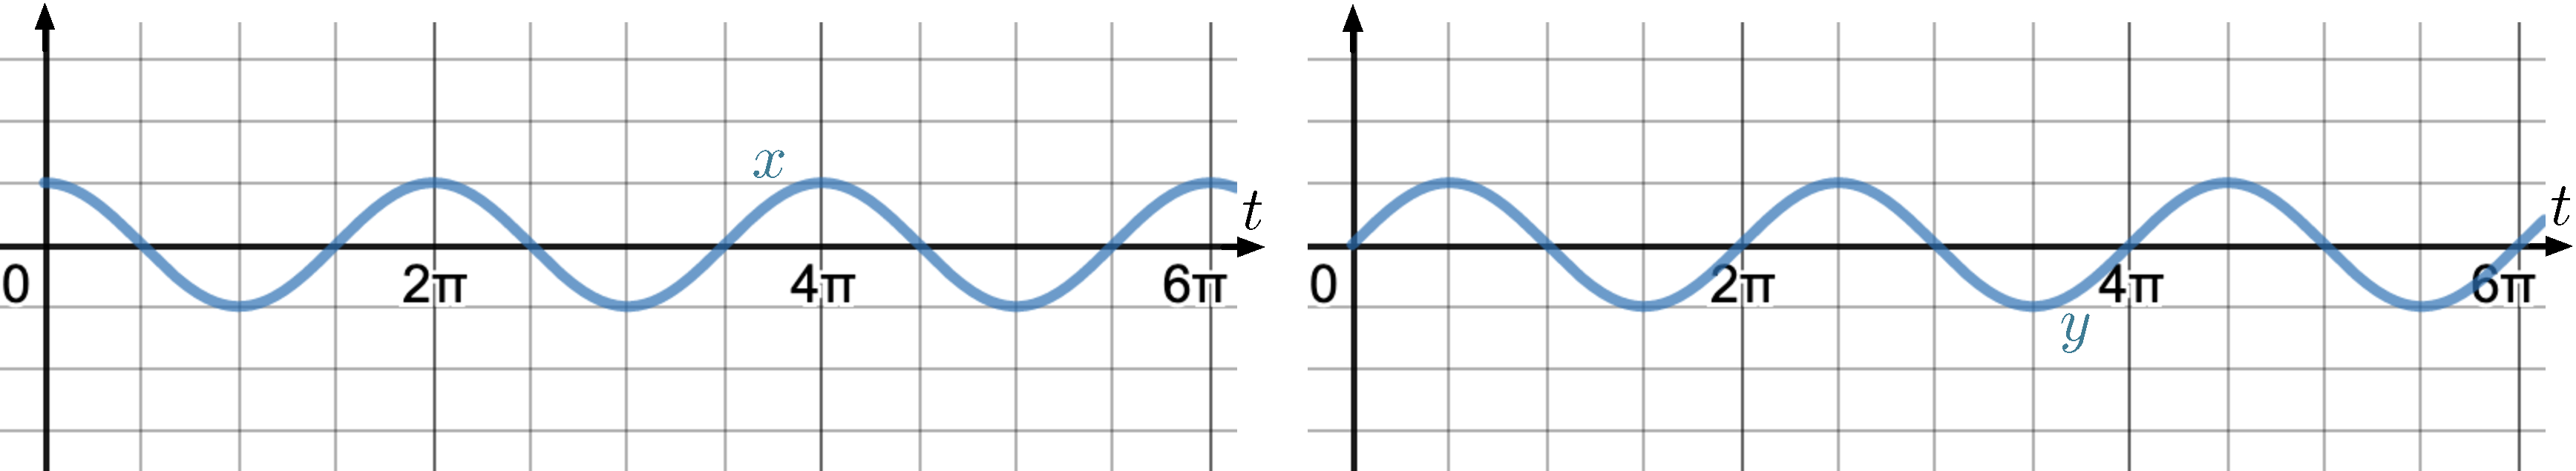
\includegraphics[width=400pt]{images/module18-sep-xy.pdf}\end{minipage}

\item \begin{minipage}{200pt}\includegraphics*[width=200pt]{images/module18-together-xy.pdf}\end{minipage}

\item \begin{minipage}{200pt}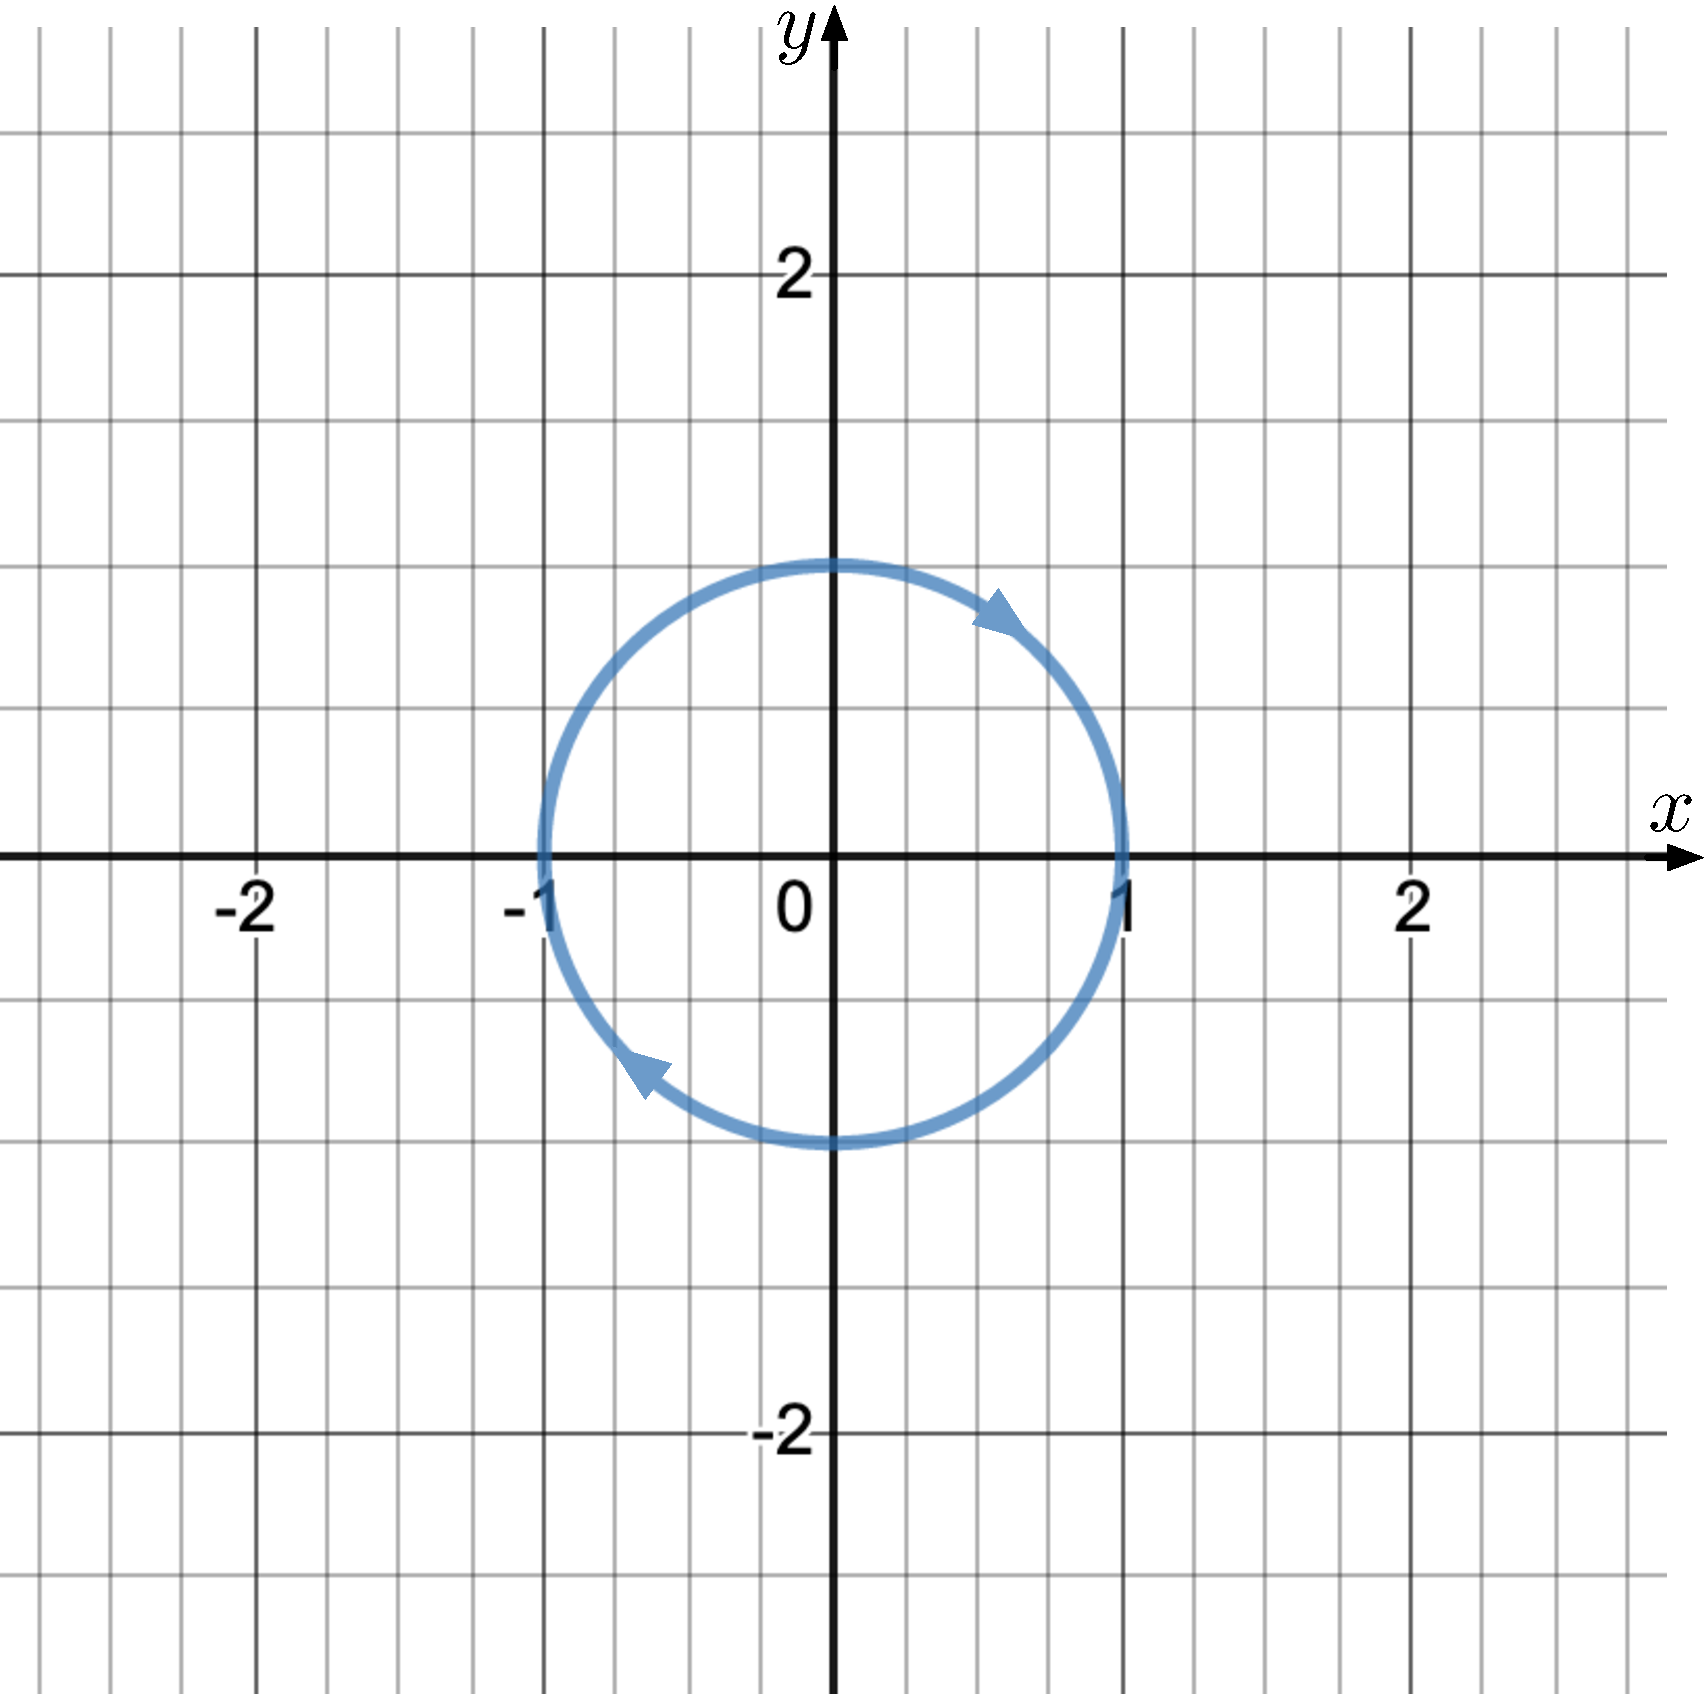
\includegraphics[height=200pt]{images/module18-phaseportrait.pdf}\end{minipage}
\end{itemize}

There is no correct answer, but the last graph gives more information on how the two quantities interact with each other, so we will focus on that type of graph.
\end{example}


The graphs in the example above are graphs of one specific solution. A phase portrait gives an idea of all possible solutions. 
\begin{example}
The last graph of the example is part of which phase portrait?

\begin{center}
\includegraphics*[width=420pt]{images/module18-possiblephaseportraits.pdf}
\end{center}

A phase portrait gives a good idea of how all solutions behave.
\end{example}

Sketching phase portraits for systems of two first-order linear ODEs is important because it gives us insight on how the two components affect each other for all solutions.

\begin{example}
Consider the problem
$$
\frac{d \, \vec{r}}{dt} = \begin{bmatrix} -2 & 3 \\ -3 & -2 \end{bmatrix} \vec{r},
$$
where the matrix $A$ has the eigenvalues and eigenvectors:
\begin{itemize}
	\item Eigenvalues $\lambda_{\pm} = -2 \pm 3i$ with eigenvectors $v_{\pm} = \begin{bmatrix} \mp i \\ 1 \end{bmatrix}$
\end{itemize}

This means that the general solution has the form
\begin{itemize}
	\item $\displaystyle \vec{r}(t) = a_1 \begin{bmatrix} -i \\ 1 \end{bmatrix} e^{(-2+3i)t} + a_2 \begin{bmatrix} i \\ 1 \end{bmatrix} e^{(-2-3i)t}$

	\item[or]
	\item $\displaystyle \vec{r}(t) = c_1 \begin{bmatrix}	 \sin(3t) \\ \cos(3t) \end{bmatrix} e^{-2t} + c_2 \begin{bmatrix}	 -\cos(3t) \\ \sin(3t) \end{bmatrix} e^{-2t}$ \\
\end{itemize}

We can use the general form and start sketching some solutions.

\begin{itemize}
	\item Let $c_1=1$ and $c_2=0$ and we obtain
	$$ \vec{r}(t) = \begin{bmatrix}	 \sin(3t) \\ \cos(3t) \end{bmatrix} e^{-2t}.$$
	
	To sketch this solution, let us start by ignoring the term $e^{-2t}$. 
	
	So we want to sketch $ \vec{r}(t) = \begin{bmatrix}	 \sin(3t) \\ \cos(3t) \end{bmatrix}$:
	\begin{center}
		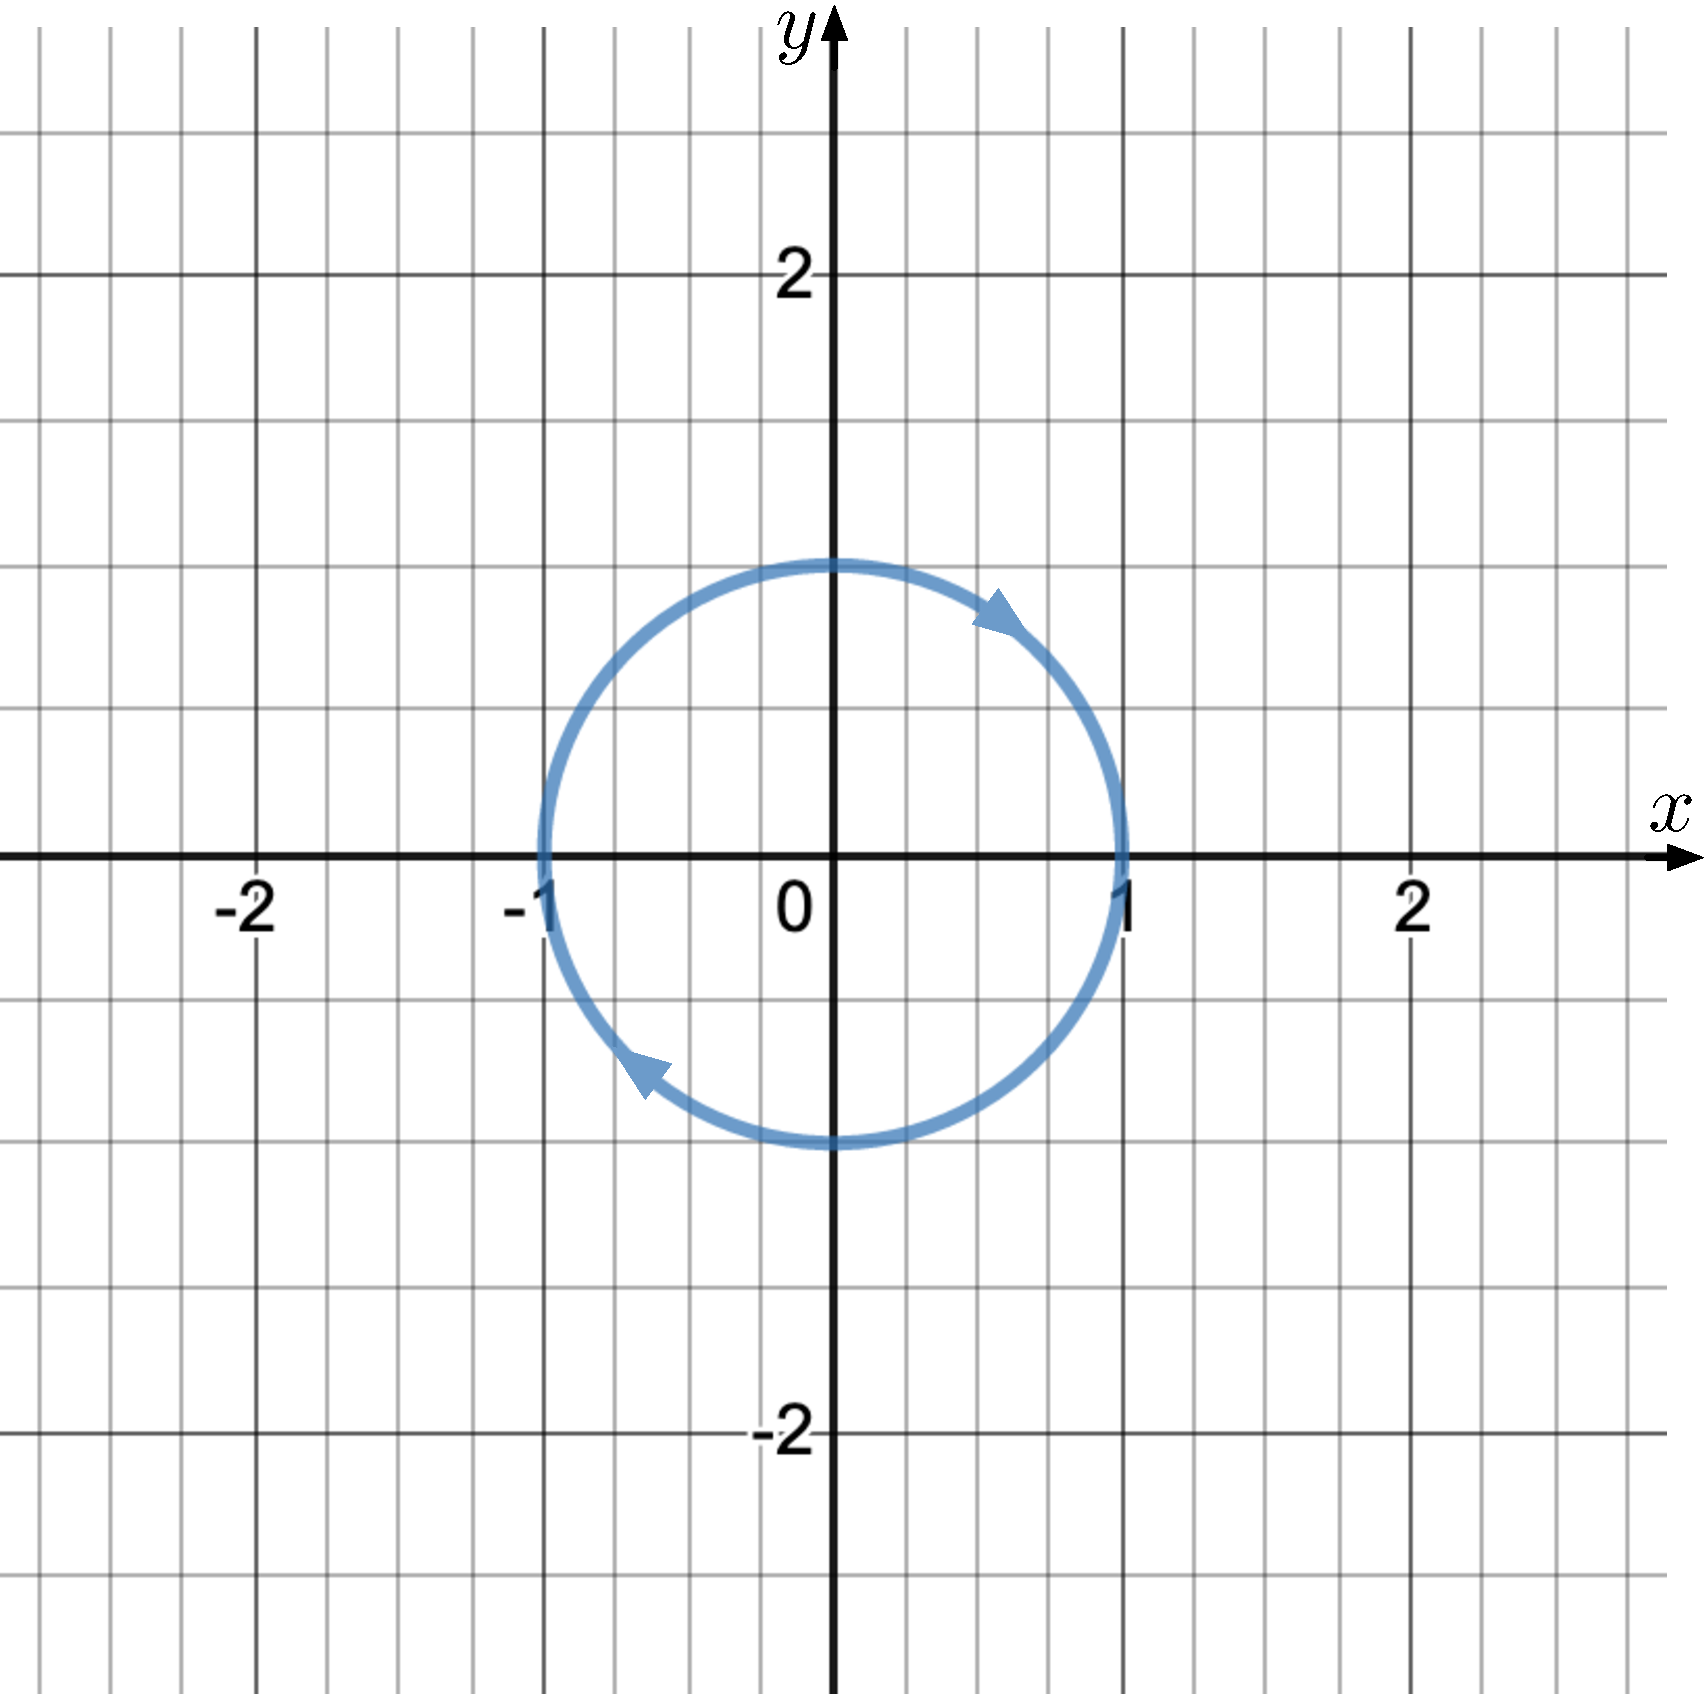
\includegraphics[height=200pt]{images/module18-phaseportrait.pdf}
	\end{center}
	
	The path is going in circles in the clockwise direction.
	
	By multiplying the solution by $e^{-2t}$, which starts at $1$ when $t=0$ and keeps decreasing towards $0$ as $t$ increases, we are creating a graph that keeps revolving around the origin as it converges towards the origin, yielding a spiral.
	\begin{center}
		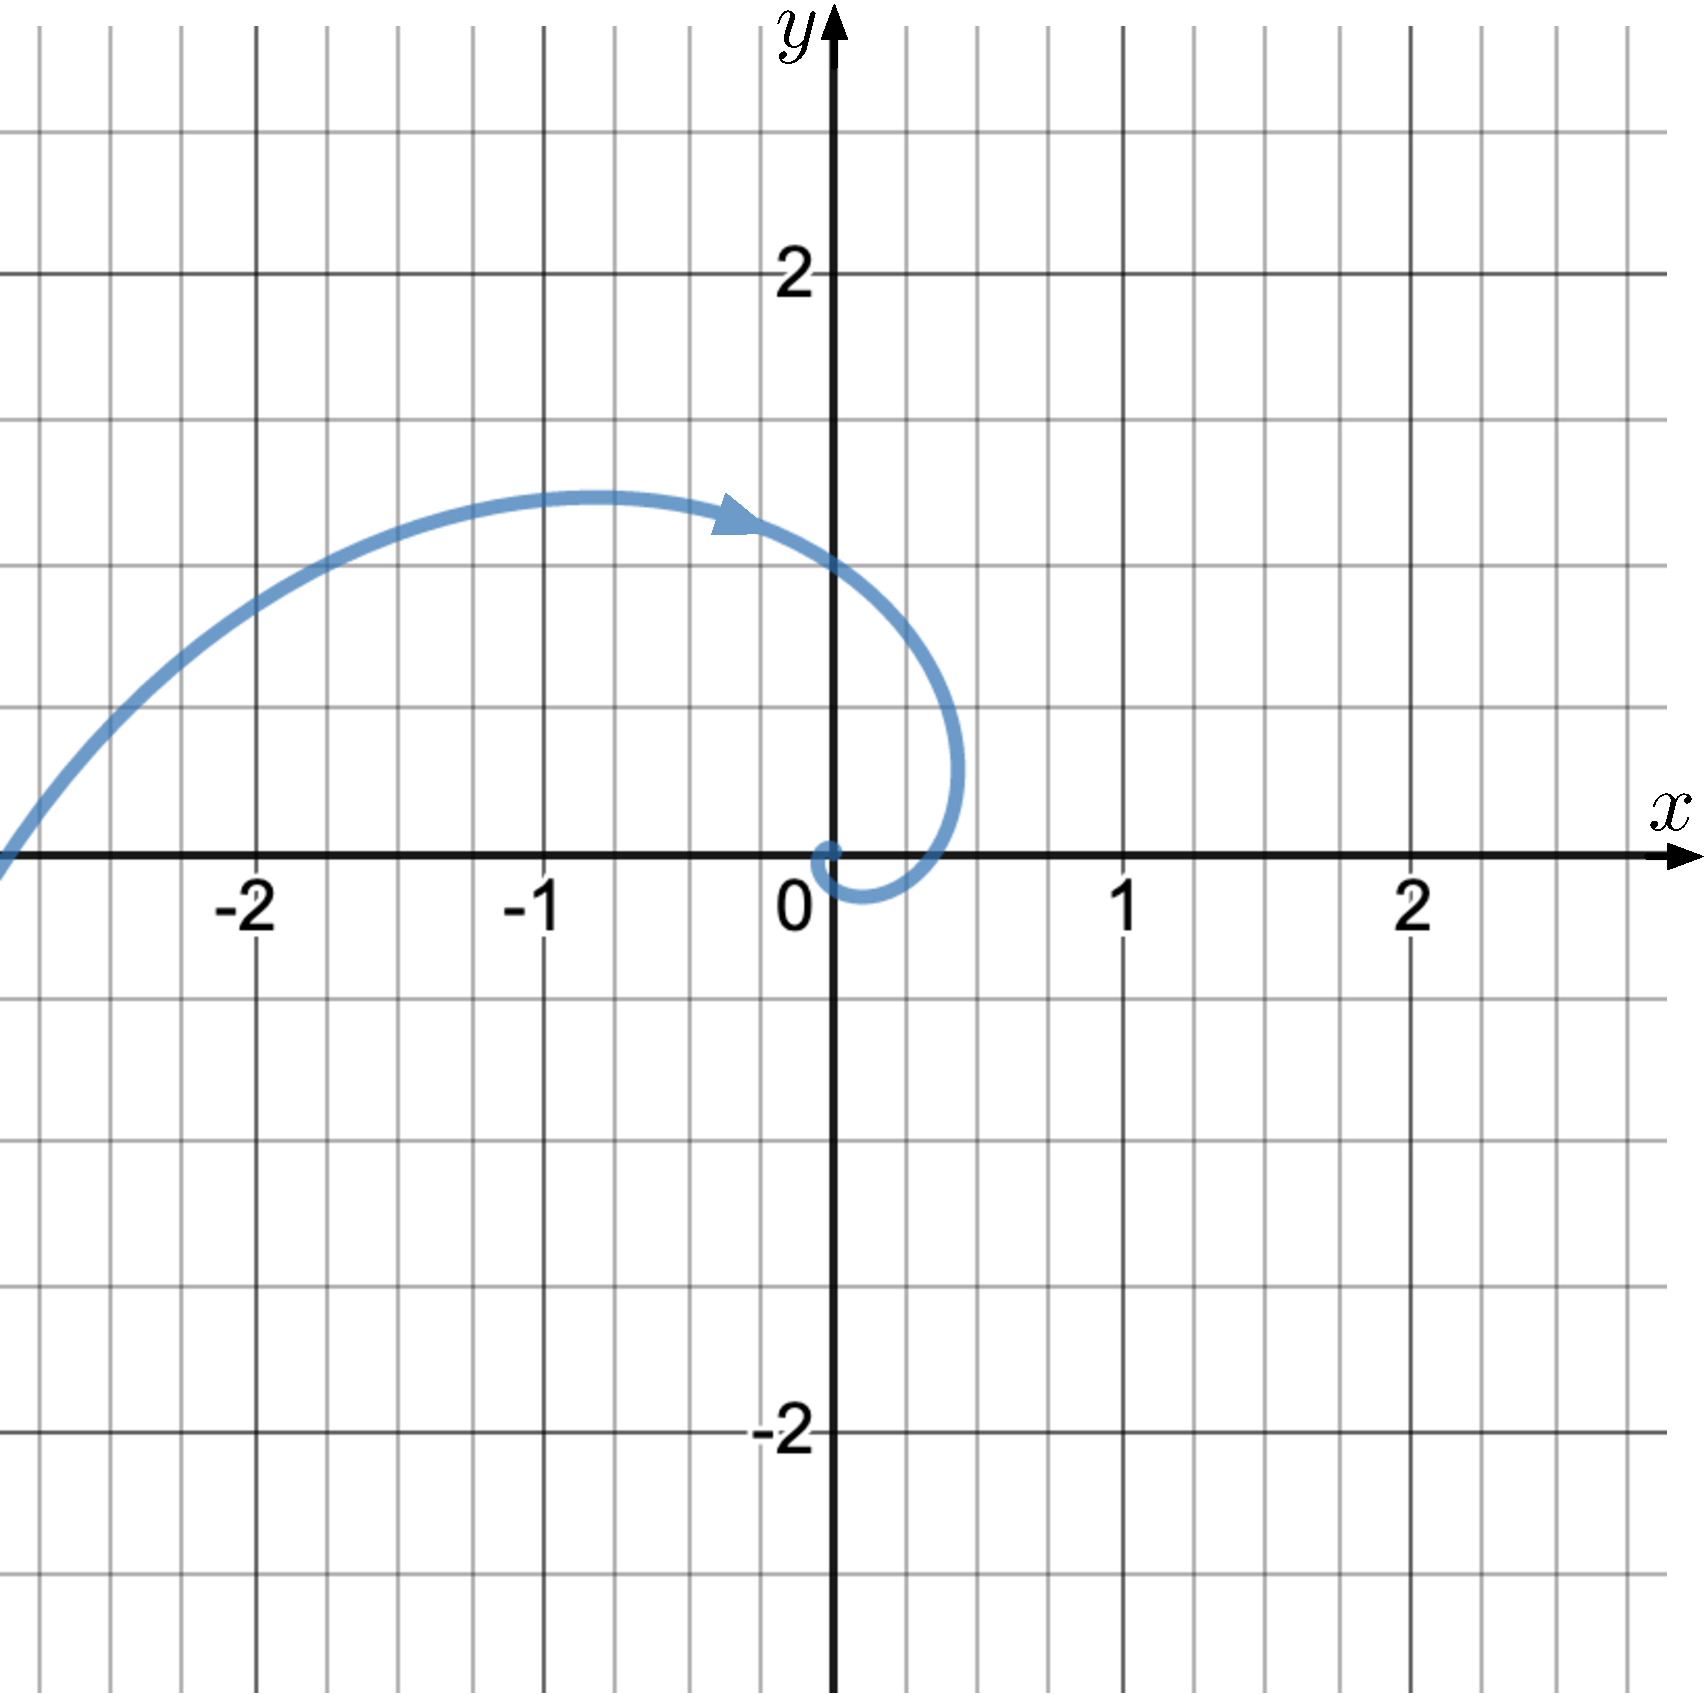
\includegraphics[height=200pt]{images/module18-spiral.pdf}
	\end{center}
	
	In this graph, we also include the graph for $t<0$. \\
	
	\item Let $c_1=-1$ and $c_2=0$ and we obtain
	$$ \vec{r}(t) = \begin{bmatrix}	 -\sin(3t) \\ -\cos(3t) \end{bmatrix} e^{-2t}$$	
	
	We add this graph to the previous one.
	\begin{center}
		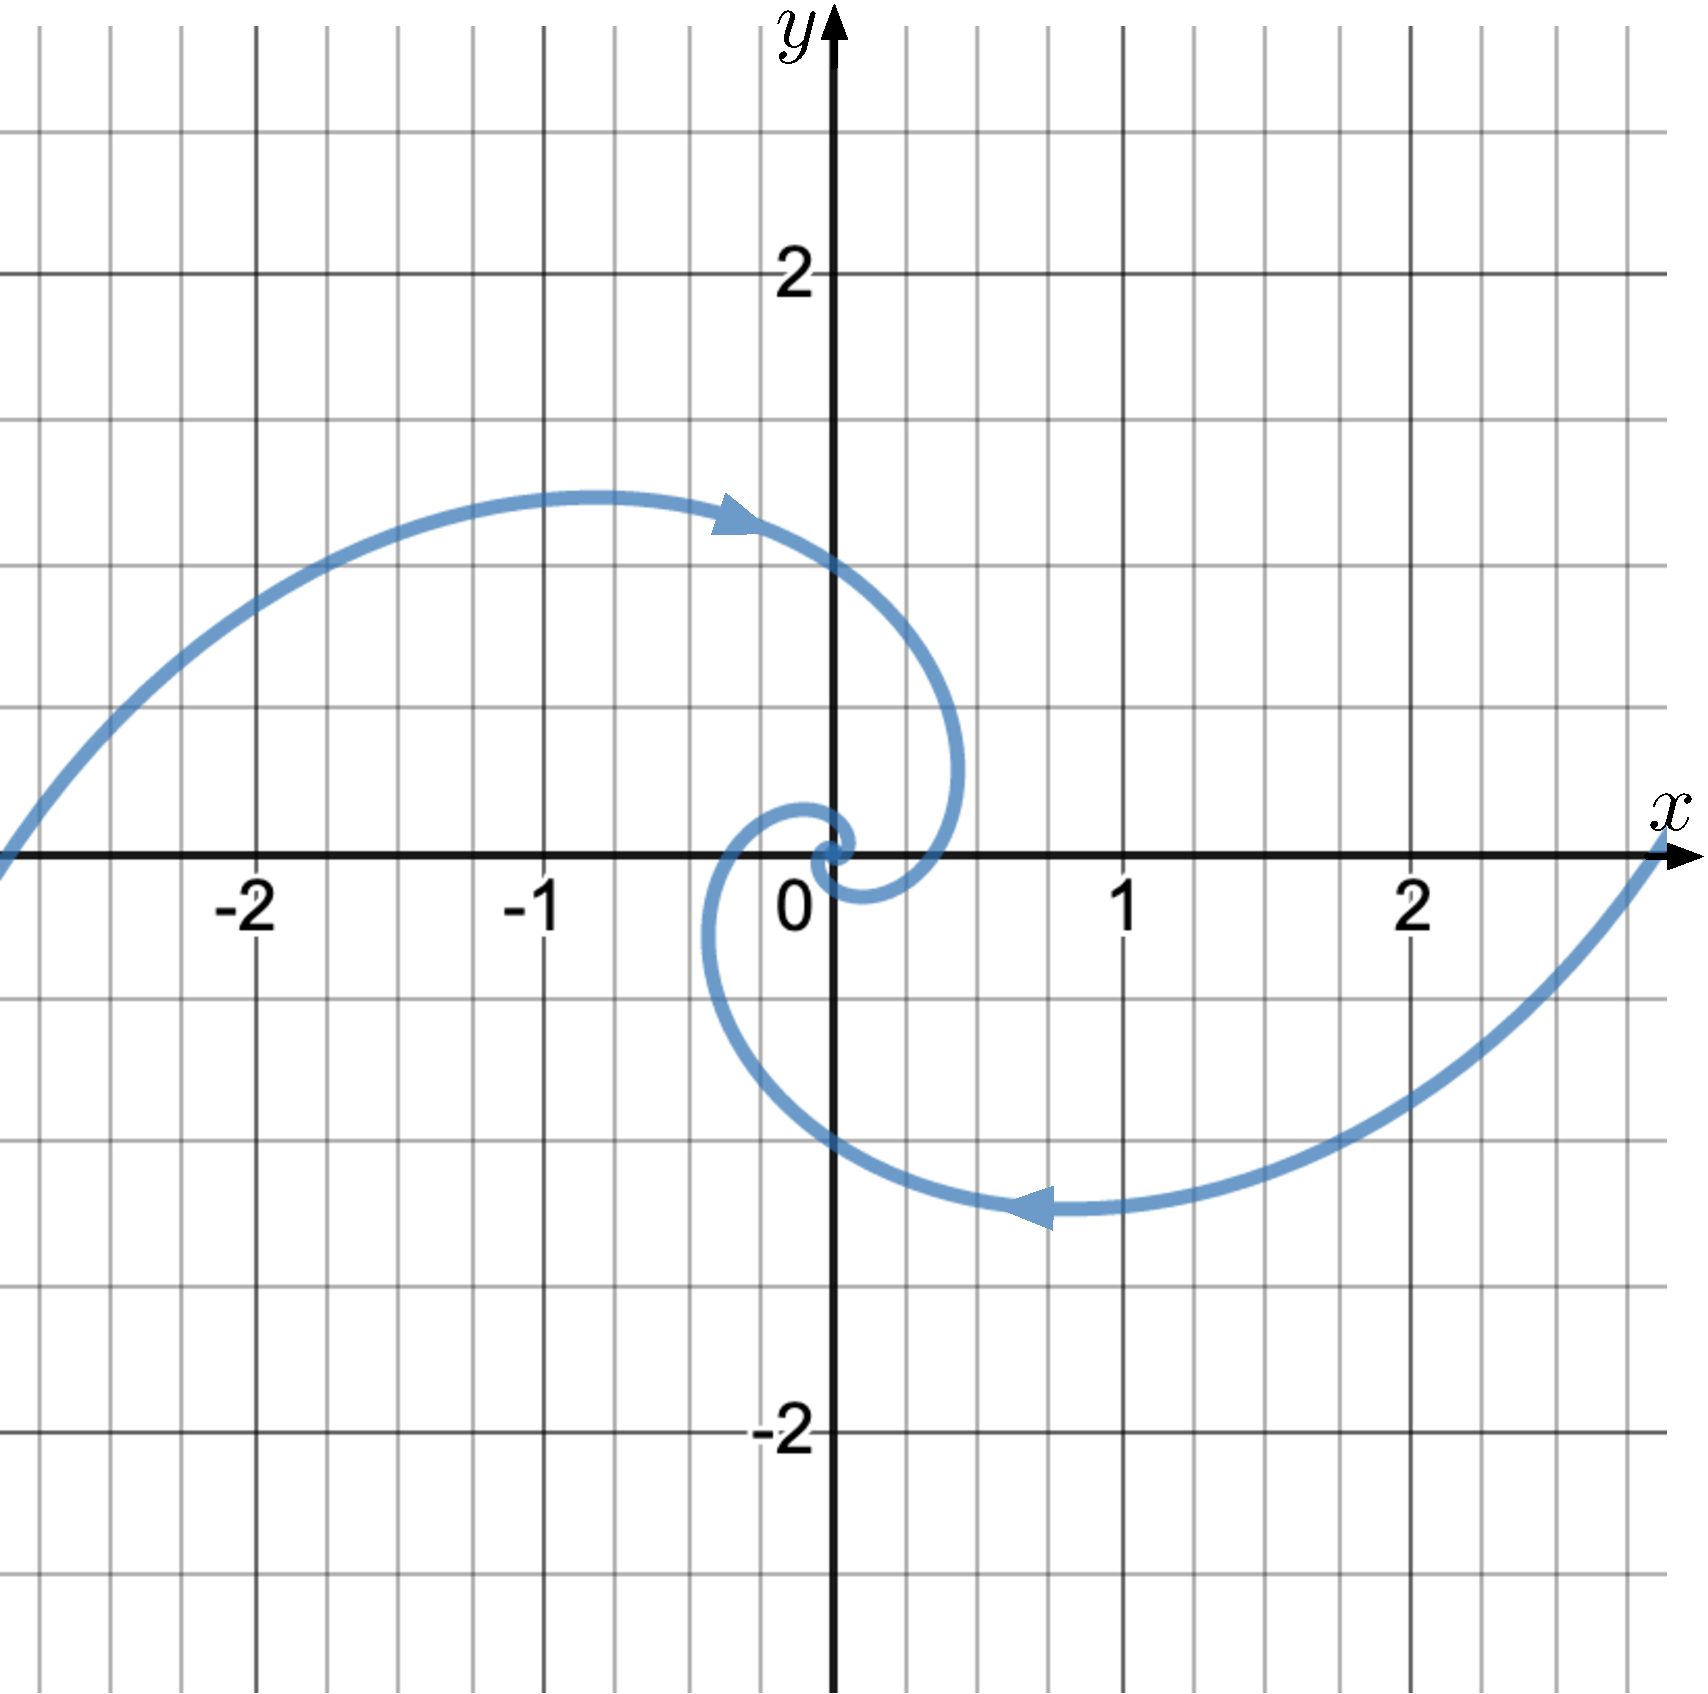
\includegraphics[height=200pt]{images/module18-spiral2.pdf}
	\end{center}
	
	\item Let $c_1=0$ and $c_2=\pm 1$ and we obtain
	$$ \vec{r}(t) = \begin{bmatrix}	 \mp \cos(3t) \\ \pm\sin(3t) \end{bmatrix} e^{-2t}.$$

	And add these to the graph:
	\begin{center}
		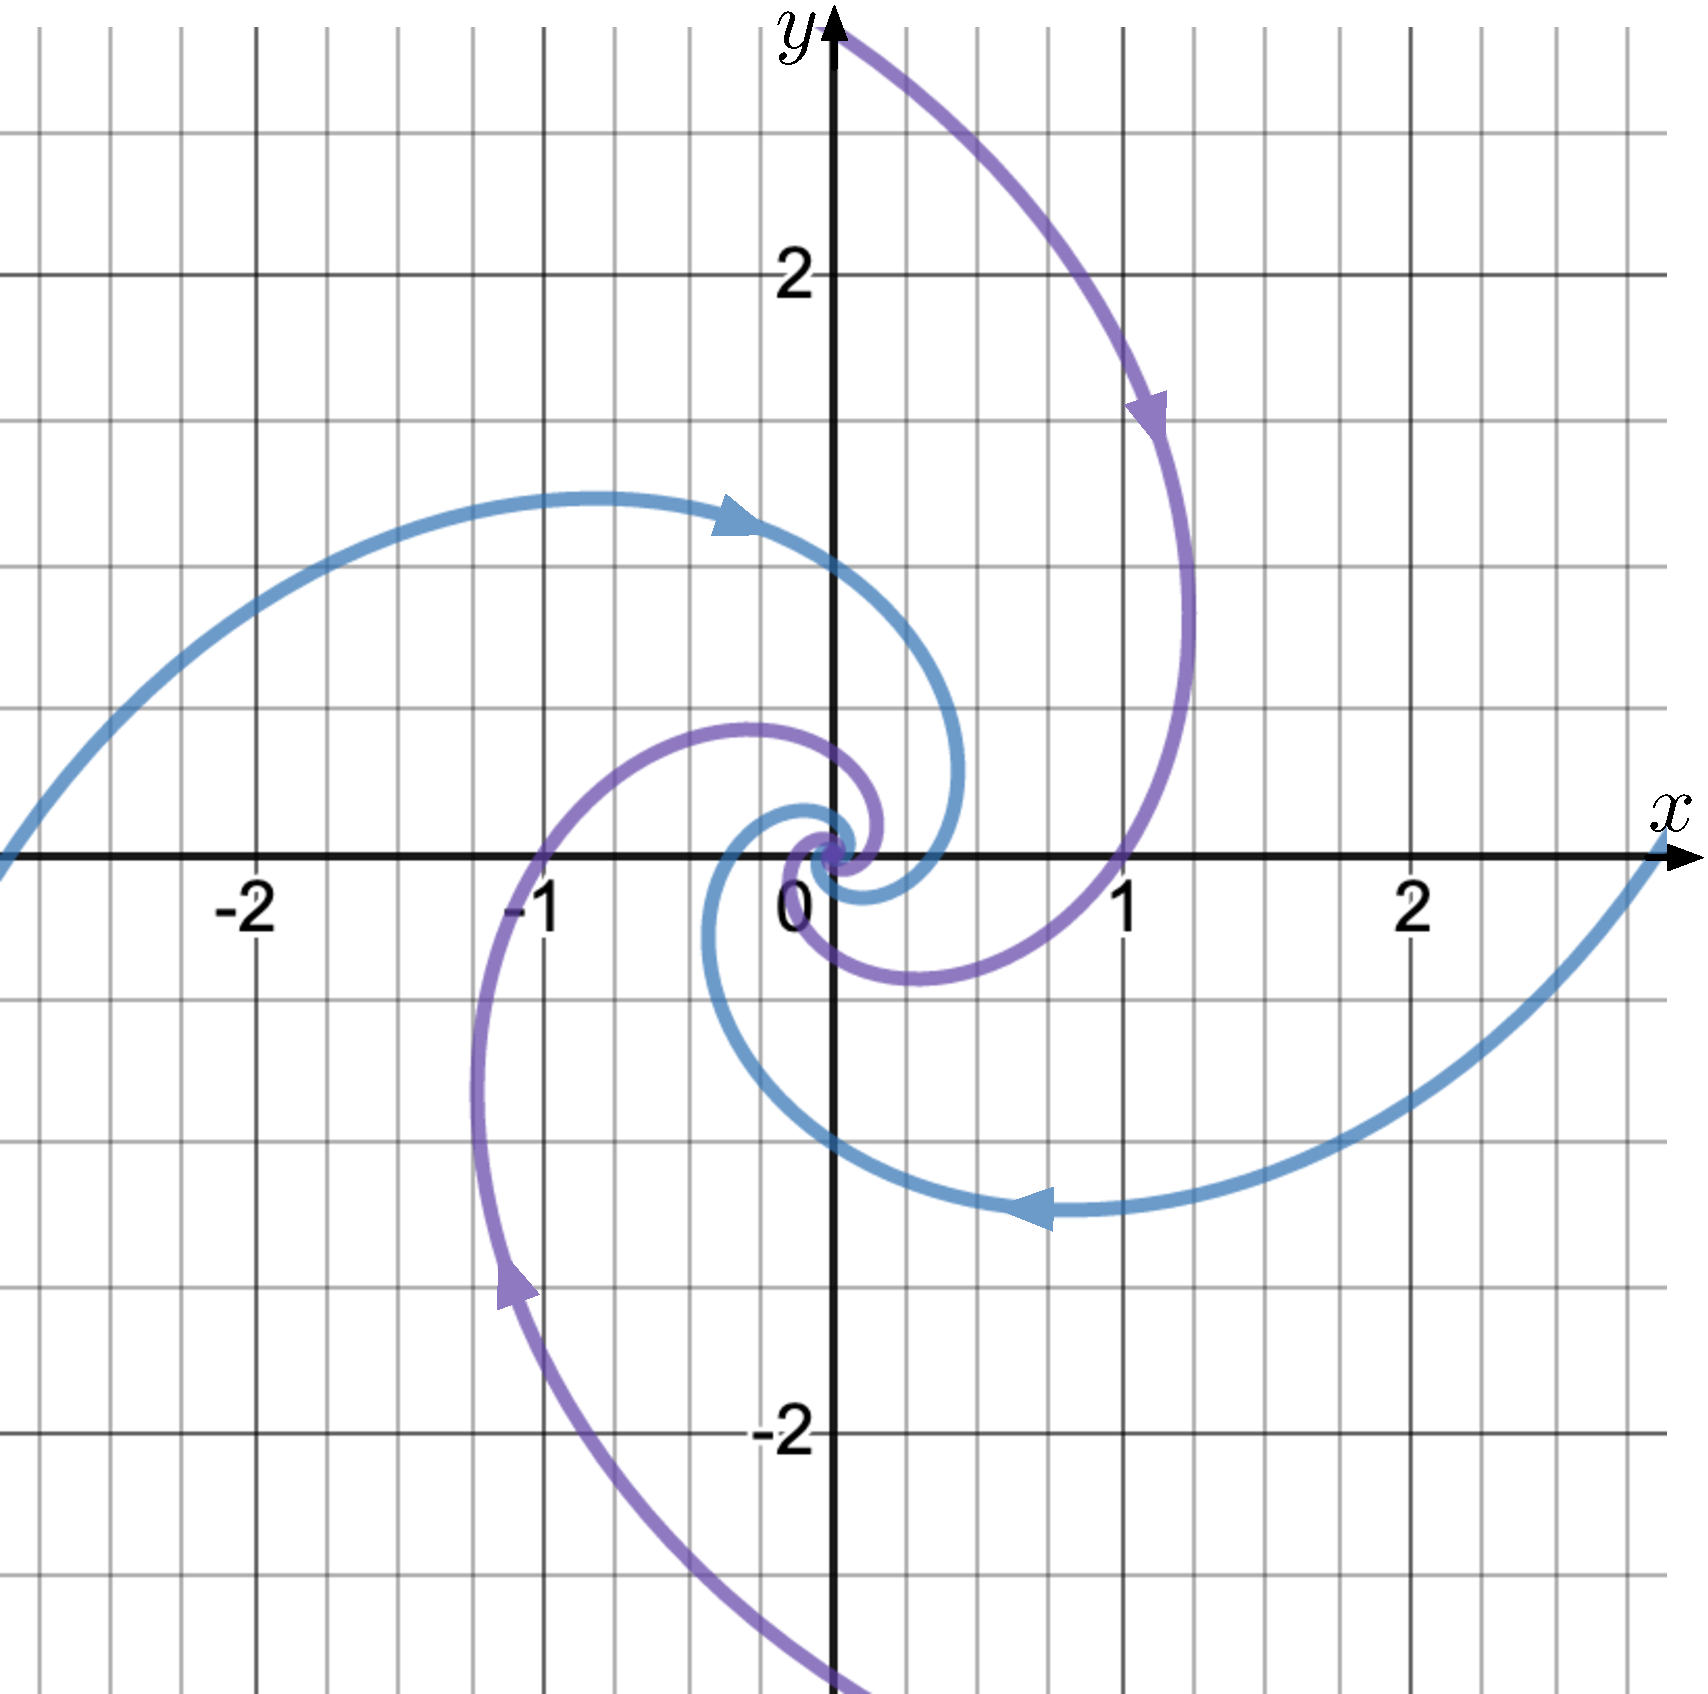
\includegraphics[height=200pt]{images/module18-spiral3.pdf}
	\end{center}

\end{itemize}

Sometimes, we need some solutions of the type $c_1=\pm 1$ and $c_2=\pm 1$ to get some different types of solutions, but we'll let you discover that on the core exercises.

These four solutions seem to give a good idea of all possible solutions: clockwise spirals converging to the origin.\\


Also observe that $\vec{r}(t) = \begin{bmatrix}0 \\ 0\end{bmatrix}$, so this system has an equilibrium solution.

This kind of equilibrium is called a \emph{spiral sink} and it is \emph{asymptotically stable}.
This means that it is a spiral and it converges to the equilibrium (the origin).
\end{example}





\begin{video}
	\begin{itemize}
		\item \qrvideo{https://youtu.be/nyI_JPDrJ_I}
		\item \qrvideo{https://youtu.be/dpbRUQ-5YWc}
	\end{itemize}
\end{video}




